%
% de Rham Kohomologie
%
\section{de~Rham-Kohomologie
\label{buch:topologie:section:drham}}
\kopfrechts{de~Rham-Kohomologie}
Die Differentialformen auf einer Mannigfaltigkeit ermöglichen eine
Konstruktion, die ganz ähnliche Eigenschaften hat wie die Vektorräume
der Simplizes, die in Abschnitt~\ref{buch:topologie:section:simplex}
konstruiert wurden.
In diesem Abschnitt wird skizziert, wie die Vektorräume der
de~Rham-Kohomologie erhalten werden können.
Man kann zeigen, dass sich auch aus der de~Rham-Kohomologie die
Euler-Charakteristik wiedergewinnen lässt.

%
% Kokettenkomplex
%
\subsection{Kokettenkomplex}
Wir betrachten eine $n$-dimensionale differenzierbare Mannigfaltigkeit
und die Vektorräume $\Omega^k(M)$ der $k$-Formen auf $M$.
Die äussere Ableitung $d$ ist eine lineare Abbildung
\[
d
\colon
\Omega^k(M) \to \Omega^{k+1}(M)
:
\alpha \mapsto d\alpha
\]
Um den Definitionsbereich etwas expliziter zu machen, schreiben wir
$d^k$ für die auf $k$-Formen definierte äussere Ableitung.
Wir erhalten also eine Folge von Vektorräumen 
\begin{equation}
\dots
\xrightarrow{\qquad\clap{$d^{k-2}$}\qquad}
\Omega^{k-1}(M)
\xrightarrow{\qquad\clap{$d^{k-1}$}\qquad}
\Omega^k(M)
\xrightarrow{\qquad\clap{$d^{k}$}\qquad}
\Omega^{k+1}(M)
\xrightarrow{\qquad\clap{$d^{k+1}$}\qquad}
\dots
\label{buch:topologie:derham:komplex}
\end{equation}
ganz ähnlich der Folge der Vektorräume der Simplizes einer
Triangulierung einer Mannigfaltigkeit.
Der Unterschied ist nur die Richtung der Pfeile, die jetzt in
Richtung aufsteigender Dimension zeigen.

Durch direkte Rechnung haben wir bereits früher eingesehen, dass die
zweimalige Anwendung der äusseren Ableitung die $k+1$-Form 0 ergibt.
Die Verkettung zweier Abbildungen in \eqref{buch:topologie:derham:komplex}
ergibt also immer $0$.
Diese Eigenschaft ist parallel zur Eigenschaft des Randoperators,
dessen Verkettungen ebenfalls immer $0$ ergeben.
Diese Ähnlichkeit rechtfertigt die folgende Definition.

\begin{definition}[Kokettenkomplex]
\index{Kokettenkomplex}%
Ein \emph{Kokettenkomplex} $(C*,d*)$ ist eine Folge $C^k$, $k\in\mathbb{Z}$
von Vektorräumen 
\[
\dots
\xrightarrow{\qquad\clap{$d^{k-2}$}\qquad}
C^{k-1}
\xrightarrow{\qquad\clap{$d^{k-1}$}\qquad}
C^k
\xrightarrow{\qquad\clap{$d^{k}$}\qquad}
C^{k+1}
\xrightarrow{\qquad\clap{$d^{k+1}$}\qquad}
\]
mit linearen Abbildungen $d^k$, dem \emph{Differential},
\index{Differential, eines Kokettenkomplexes}%
derart, dass $d^{k+1}\circ d^k=0$ für alle $k$.
\end{definition}

Die Vektorräume der $k$-Formen bilden also den Kokettenkomplex
$(\Omega^k(M),d^k)$ der $k$-Formen,
mit der äusseren Ableitung als Differential.
Natürlich ist $\Omega^k(M)=0$ für $k<0$ oder $k>n$ zu wählen.

%
% Kozyklen und Koränder
%
\subsection{Kozyklen und Koränder}
Bei einem Kettenkomplex waren die Zyklen von besonderem Interesse,
in der Homologietheorie wurden dann aber diejenigen Zyklen ignoriert,
die als Rand entstehen konnten.

\begin{definition}[Kozyklen und Koränder]
Sei $(C*,d*)$ ein Kokettenkomplex.
Ein $z\in C^k$ mit $d^kz=0$ heisst \emph{Kozyklus}.
\index{Kozyklus}%
Der Kern von $d^k$ wird mit
\[
\ker d^k = \{ z\in C^k\mid d^kz=0\}
=
Z^k(C)
\]
bezeicnnet.
Ist $z\in C^k$ und gibt es $b\in C^{k-1}$ mit $d^{k-1}b=z$, dann 
heisst $z$ ein \emph{Korand}.
\index{Korand}%
Die Menge der Koränder in $C^k$ ist also das Bild
\[
\operatorname{im}d^{k-1}
=
\{
d^{k-1}b\mid b\in C^{k-1}
\}
\]
von $d^{k-1}$.
\end{definition}

Im folgenden betrachten wir den Kokettenkomplex $(\Omega^*(M),d^*)$ 
der Differentialformen auf einer $n$-dimensionalen Mannigfaltigkeit.
Da für alle $n$-Formen $\omega$ gilt $d^n\omega=0$ besteht die Menge
der $n$-dimensionalen Kozyklen aus ganz $\Omega^n(M)$.
Für eine orientierbare, zusammenhängende Mannigfaltigkeit lässt sich
sogar eine explizite Beschreibung aller Kozyklen angeben, sie sind
alle Vielfache der Volumenform.

Für $k=0$ ist die Menge Kozyklen ebenfalls einfach zu bestimmen.
Sie besteht aus denjenigen $0$-Formen, deren Ableitung verschwindet.
0-Formen sind aber einfach Funktionen.
Die Menge der Kozyklen besteht daher einfach aus den Konstanten.
Für eine zsammenhängende Mannigfaltigkeit ist also
$Z^0(M)=\mathbb{R}$.
Die Menge der Koränder ist ebenfalls einfach: da $\Omega^{-1}(M)=0$ ist,
muss auch $B^0(M)=0$ sein.

%
% Definition der Kohomologiegruppen
%
\subsection{Definition der Kohomologiegruppen}
Die Definition der Homologievektorräume ging davon aus, dass Ränder
nichts über die Topologie einer Mannigfaltigkeit verraten, weil sie
sich zusammeziehen lassen.
Wir erwarten eine ähnliche Eigenschaft auch für den Kokettenkomplex
der $k$-Formen und definieren daher die Kohomologiegruppen wie 
folgt.

\begin{definition}
Sie $M$ eine differenzierbare $n$-dimensionale Mannigfaltigkeit, dann
ist die $k$-te \emph{de~Rham-Kohomologiegruppe} der Vektorraum
\index{de Rham-Kohomologiegruppe}%
\[
H^k(M)
=
Z^k(M) / B^k(M).
\]
\end{definition}

Für eine zusammenhängende $n$-dimensionale Mannigfaltigkeit wissen wir
bereits, dass $Z^0(M)\equiv\mathbb{R}$ und $B^0(M)=0$, also ist
\[
H^0(M) = Z^0(M) / B^0(M) = \mathbb{R}.
\]
Falls $M$ aus mehreren Komponenten besteht, ist ein Kozyklus eine
Funktion, die in jeder Komponente konstant ist.
Die Kohomologiegruppe $H^0(M)$ ist also ein Vektorraum mit sovielen
Dimensionen, wie die Mannigfaltigkeit Kompoenten hat.

%
% Integration über $k$-Simplizes
%
\subsubsection{Integration über $k$-Simplizes}
Die Elemente der Kohomologiegruppe $H^k(M)$ quantifizieren, warum
ein Kozyklus $\alpha\in \Omega^k(M)$ nicht als Korand $\alpha=d^{k-1}\beta$
geschrieben werden kann.
Dazu betrachtet man ein in die Mannigfaltigkeit eingebettetes
$k+1$-dimensionales Simplex $S\subset M$.
Nach dem allgemeinen Satz von Stokes ist das Integral über den Rand von
$S$
\[
\int_{\partial S} \alpha
=
\int_{\partial S} d\beta
=
\int_{\partial\partial S}\beta
=
0.
\]
Damit $\alpha$ ein Korand ist, müssen alle diese Integrale verschwinden.

Tatsächlich kann man zeigen, dass die Integration von $k$-Formen über
die Simplizes einer Triangulation einer Mannigfaltigkeit viel mehr
liefert als nur eine Analogie zwischen den Konstruktionen der
simplizialen Homologie und der de~Rham-Kohomologie.
Es stellt sich heraus, dass der Kohomologievektorraum $H^k(M)$
der duale Vektorraum zum Homologievektorraum $H_k(M)$ ist.
Schreibt man
\[
\langle \alpha, c \rangle
=
\int_c \alpha
\]
für das Integral einer $k$-Form über eine $k$-dimensionale Kette, dann
lässt sich der allgemeine Satz Stokes als
\[
\langle d\alpha, c\rangle
=
\langle \alpha,\partial c\rangle
\qquad
\alpha\in \Omega^k(M),\; c\in C_{k+1}
\]
schreiben.
Dies bedeutet, dass $d$ und $\partial$ duale Operatoren sind.

%
% Euler-Charakteristik
%
\subsubsection{Euler-Charakteristik}
Aus der oben angedeuteten aber nicht bewiesenen Tatsache, dass die
Kohomologiegruppen orientierbarer Mannigfaltigkeiten die dualen
Vektorräume der Homologievektorräume sind, bedeutet auch, dass die 
Dimensionen übereinstimmen.
Somit gilt auch der folgende Satz.

\begin{satz}
Ist $M$ eine zusammenhängende, orientierbare Mannigfaltigkeit, dann ist
\[
\chi(M)
=
\sum_{k=0}^n (-1)^k \dim H^k(M).
\]
\end{satz}

Die früher mit Simplizes kombinatorisch definierte Euler-Charakteristik
kann also auch durch Betrachtung von Differentialformen untersucht
werden.

%
% Beispiele
%
\subsection{Beispiele}
Ein vielen Fällen kann man den Vektorraum der Differentialformen,
der Kozyklen und der Koränder vollständig charakterisieren und damit
auch die Kohomologiegruppen berechnen.

%
% Kohomologie eines zusammenziehbaren Raumes
%
\subsubsection{Kohomologie eines zusammenziehbaren Raumes}
Das Poincaré-Lemma besagt, dass auf einer zusammenziehbren Menge
$M$ für jede $k$-Form $\alpha$ mit $d\alpha=0$ eine $k-1$-Form
$\beta$ gefunden werden kann, mit $d\beta = \alpha$.
Wegen $d\alpha=0$ ist $\alpha\in Z^k(M)$ ein Zyklus.
Ausserdem ist $d\beta\in \operatorname{im}d^k = B^k(M)$ ein Rand.
Das Poincaré-Lemma sagt als, dass jeder Zyklus auch ein Rand ist,
oder $Z^k(M) = B^(K)$.
Somit ist der Quotient
\[
H^k(M)
=
Z^k(M) / B^k(M)
=
\{0\}
\]
der 0-dimensionale Vektorraum.
Alle Kohomologiegruppen verschwinden also.

%
% Eindimensionale Mannigfaltigkeiten
%
\subsubsection{Eindimensionale Mannigfaltigkeiten}
Die eindimensionalen zusammenhängenden Mannigfaltigkeiten sind leicht
zu klassifizieren.
Lokal sehen sie wie ein $\mathbb{R}$ aus.
Ausgehend von einem Punkt kann man sich also nur in zwei Richtungen
bewegen.
Eine Kurve $\mathbb{R}\to M$ mit Tangentialvektor $\ne 0$ in der
Mannigfaltigkeit folgt ihr, ohne umzukehren.
Indem wir eine Metrik verwenden, können wir auf zwei Möglichkeiten
reduzieren: die Kurve ist eine injektive Abbildung, d.~h. die Mannigfaltigkeit
enthält eine Komponenten, die zu $\mathbb{R}$ diffeomorph ist,
oder die Kurve kehrt zu einem Punkt zurück, d.~h. die Mannigfaltigkeit
enthält eine Komponente, die zu einer Kreislinie diffeomorph ist.

Die Komponente $\mathbb{R}$ ist zusammenziehbar, also ist $H^1(\mathbb{R})=0$.

Zur genaueren Untersuchung von $S^1$ schreiben wir 
\[
S^1
=
\mathbb{R}/\mathbb{Z},
\]
d.~h. Punkte in $\mathbb{R}$ werden miteinander identifiziert, wenn
sie sich um eine ganze Zahl unterscheiden.
Funktionen $\beta\colon S^1\to\mathbb{R}$ sind also periodische Funktionen 
mit $\beta(x+1)=\beta(x)$.

Wegen $n=1$ sind
alle $1$-Formen auf $S^1$ Kozyklen, $Z^1(S^1)=\Omega^1(S^1)$.
Zur Bestimmung von $H^1(S^1)$ ist jetzt zu unterscuhen,
welche $1$-Formen keine Koränder sind.
Ein Korand $\alpha$ ist eine 1-Form, welche durch Ableitung einer
Funktion $\beta$ auf $S^1$ entsteht, sie muss also von der Form
$\alpha=\beta'(x)\,dx$, wobei $f$ eine periodische Funktion ist.
Durch Integration über eine Periode folgt
\[
\int_{S^1} \alpha
=
\int_{S^1} d\beta
=
\int_{\partial S^1} \beta
=
0.
\]
Eine $1$-Form ist also genau dann ein Korand, wenn das Integral
über $S^1$ verschwindet.
Es folgt, dass
\[
\int_{S^1}
\colon
\Omega^1(S^1)\to \mathbb{R}
:
\alpha
\mapsto
\int_{S^1}\alpha
\]
eine lineare Abbildung ist, die als Kern genau
$B^1(S^1)=\operatorname{im}d^0$ hat.
Somit ist
\[
H^1(S^1)
=
Z^1(S^1) / B^1(Z)
=
\mathbb{R}.
\]
Die Euler-Charakteristik ist
\[
\chi(S^1)
=
\sum_{k=0}^1 (-1)^k\dim H^k(S^1)
=
1-1
=
0,
\]
wie man auch mit einer Triangulation, die in Dimension 1 natürlich nur
aus Punkten und Strecken besteht, nachprüfen kann.

%
% Torus
%
\subsubsection{Torus}
%
% fig-toruspfade.tex
%
% (c) 2025 Prof Dr Andreas Müller
%
\begin{figure}
\centering
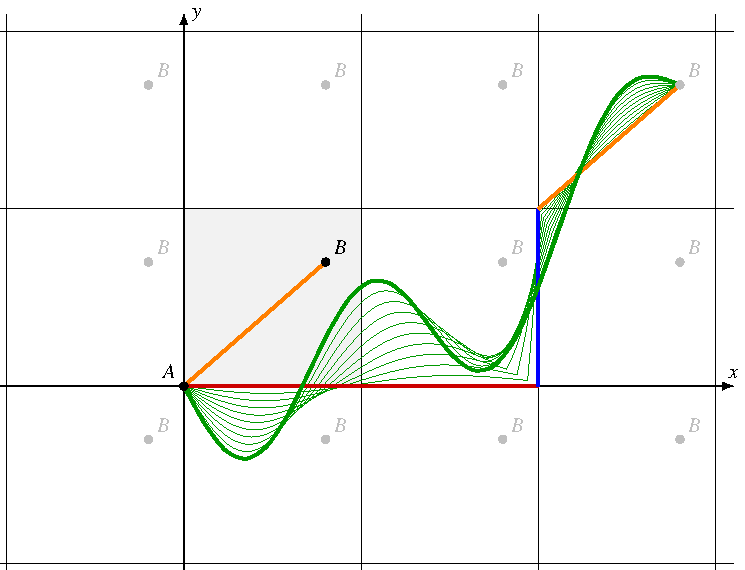
\includegraphics{chapters/120-topologie/images/toruspfade.pdf}
\caption{Ein zweidimensionaler Torus $T$ wird beschrieben als die
Punkte der zweidimensionalen Ebene, die aber als gleich betrachtet
werden, wenn sich ihre Koordinaten um eine Ganzzahl unterscheiden.
Alle Punkte $B$ in der Ebenen stellen also den gleichen Punkt auf dem
Torus dar.
Ein Weg von $A$ zu $B$ im Torus ist ein Weg von $A$ zu einem beliebigen
Repräsentanten von $B$ in der Ebene.
Jeder solche Pfad ({\color{darkgreen}grün}) kann zerlegt werden in
einen Pfad, der zunächst aus Segmenten ganzzahliger Länge parallel
zur $x$-Achse ({\color{darkred}rot}) bzw.~zur $y$-Achse
({\color{blue}blau}) besteht, gefolgt von einem Segment zum Punkt
$B$ in einem einzelnen Quadrat der Ebene ({\color{orange}orange}).
\label{buch:topologie:kohomologie:fig:toruspfade}}
\end{figure}

Der zweidimensionale Torus $T$ kann beschrieben werden als die
Menge $\mathbb{R}^2$, in der Punkte miteinander identifiziert
werden, die sich genau um $1$ in $x$- bzw.~$y$-Richtung unterscheiden.
Man definiert also eine Äquivalenzrelation $\sim$ durch
\[
(x+1,y \sim (x,y) \sim (x,y+1).
\]
Dann ist der Torus die Menge
\[
T
=
\{ (x,y) \mid x,y\in\mathbb\}
/
\sim.
\]
Diese Situation ist in
Abbildung~\ref{buch:topologie:kohomologie:fig:toruspfade}
dargestellt .

Ein zweidimensionaler Torus $T$ ist zusammenhängend, daher ist
$H^0(T)\mathbb{R}$ eindimensional.

Um die eindimensionalen Kohomologiegruppen zu berechnen, muss man
untersuchen, welche eindimensionale Kozyklen auch Ränder sind.
Sei also $\alpha\in \Omega^1(T)$ mit der Eigenschaft, dass $d\alpha=0$
ist.
Wir können $\alpha = f(x,y)\,dx + g(x,y)\,dy$ schreiben, die äussere Ableitung
ist dann
\[
d\alpha
=
\frac{\partial f}{\partial y}\,dy\wedge dx
+
\frac{\partial g}{\partial y}\,dx\wedge dy
=
\biggl(\frac{\partial g}{\partial y}-\frac{\partial f}{\partial x}\biggr)
\,dx\wedge dy.
\]
Ein Kozyklus zeichnet sich daher dadurch aus, dass
\begin{equation}
\frac{\partial g}{\partial y}-\frac{\partial f}{\partial x}
=
0
\label{buch:topologie:derham:eqn:integrabilitaet}
\end{equation}
ist.
Der Satz von Green besagt, dass unter Voraussetzung
\eqref{buch:topologie:derham:eqn:integrabilitaet}
das Wegintegral
\[
\int_\gamma \alpha
\]
für einen Weg zwischen zwei Punkten auf $\mathbb{R}^2$ nicht vom Weg
in $\mathbb{R}^2$ abhängt.

Zwei Punkte in $T$ können durch verschiedene Punkte in
$\mathbb{R}^2$ repräsentiert werden, die sich durch eine Ganzzahl
in jeder Koordinaten unterscheiden.
Zwischen den Punkten $A$ und $B$ in $T$ gibt es daher viele Wege.
In Abbildung~\ref{buch:topologie:kohomologie:fig:toruspfade} sind
mehrere Pfade dargestellt.
Der orange Pfad führt von $A=(0,0)$ zum Punkt $B$ im Einheitsquadrat.
Der grüne Pfad führt von $A=(0,0)$ zu dem weiter entfernten
Repräsentanten, dessen $x$- und $y$-Koordinaten um 2 bzw.~1 grösser
sind.
Dieser zweite Pfad kann in einen Pfad deformiert werden, der erst
zwei Einheiten lang der $x$-Achse folgt ({\color{darkred}rotes}
Teilstück), dann eine Einheit in Richtung der $y$-Achse verläuft
({\color{blue}blaues} Teilstück), um dann dem {\color{orange}orangen}
Teilstück bis zum Punkt $B$ zu folgen.

Wir wählen jetzt $A=(0,0)$ und versuchen eine Funktion $\beta$ zu
konstruieren, so dass $d\beta =\alpha$ ist.
Dazu müssen wir den Funktionswert $\beta(x,y)$ bestimmen.
Zu diesem Zweck integrieren wir über einen Weg in $T$ von $A$ nach
$B=(x,y)$, wobei wir annehmen dürfen, dass $x,y\in[0,1)$.
Jedem Weg von $A$ nach $B$ in $T$ entspricht ein Weg von $(0,0)$
zu einem Punkt $(x+k,y+l)$ in $\mathbb{R}$.
Der Weg in $T$ ist also deformierbar in einen Weg
zunächst von $(0,0)$ nach $(k,0)$ dann nach $(k,l)$ und schliesslich
zu $(x,y)$.

Wenn es die Funktion $\beta$ gibt, dann muss man sie durch Integration
entlang eines beliebigen Wegs in $T$ erhalten können.
Wie Abbildung~\ref{buch:topologie:kohomologie:fig:toruspfade}
illustriert lässt sich ein solcher Weg immer zerlegen in 
$k$ Segmente der Länge $1$ in $x$-Richtung ({\color{darkred}rot})
und $l$-Segmente der Länge $1$ in $y$-Richtunge ({\color{blue}blau})
gefolgt vom direkten Pfad im Einheitsquadrat von $(0,0)$ zu $(B)$
({\color{orange}}).
Die Funktion $\beta$ im Punkt $B$ muss daher
\begin{align*}
\beta(B)
&=
\beta(B) - \beta(A)
=
\int_{{\color{darkgreen}\gamma_{AB}}} d\beta
=
\int_{{\color{darkgreen}\gamma_{AB}}} \alpha
\\
&=
k\int_{(0,0)}^{(1,0)}\alpha
+
l\int_{(0,0)}^{(0,1)}\alpha
+
\int_{(0,0)}^{\color{orange}(B)}\alpha
\end{align*}
für beliebige $k,l\in\mathbb{Z}$.
Dies ist nur dann möglich, wenn die beiden ersten Integrale verschwinden.
Die Abbildung
\[
H^1(T)
\to
\mathbb{R}^2
:
\alpha
\mapsto
\biggl(
\int_{(0,0)}^{(1,0)}
\alpha,
\int_{(0,0)}^{(0,1)}
\alpha
\biggr)
\]
ist eine lineare Abbildung, deren Kern genau aus den Korändern besteht.
Es folgt daher, dass
\[
H^1(T) = \mathbb{R}^2
\]
zweidimensional ist.

Weiter ist $H^2(T)=\mathbb{R}$, so dass die Euler-Charakteristik des Torus
\[
\chi(T)
=
\dim H^0(T) - \dim H^1(T) + \dim H^2(T)
=
1-2+1
=
0.
\]
Dies stimmt überein mit der Euler-Charakteristik, die mit einer Triangulation
berechnet wurde.

%
% Kugel
%
\subsubsection{Kugel}
Auf einer zweidimensionalen Kugel $S^2$ sind alle Pfade zwischen zwei
Punkten ineinander deformierbar.
Für eine 1-Form $\alpha$ können wir daher die Funktion $\beta$ durch
\[
\beta(B)
=
\int_{\gamma_{AB}} \alpha
\]
definieren, wobei $\gamma_{AB}$ ein beliebiger Pfad von $A$ nach $B$.

Zwei verschiedenen Pfaden $\gamma_{AB}$ und $\tilde{\gamma}_{AB}$
lassen sich ineinander deformieren, es gibt daher eine Abbildung
\[
H
\colon
[0,1]\times[0,1] \to S^2
\qquad\text{mit}\qquad
H(t,s)
=
\begin{cases}
\gamma_{AB}(t)          &\qquad s=0\\
\tilde{\gamma}_{AB} (t) &\qquad s=1.
\end{cases}
\]
Da $H$ für $t=0$ und $t=1$ konstant ist, ist das Integral 
\begin{align*}
\int_{\gamma_{AB}} \alpha
-
\int_{\tilde{\gamma}_{AB}} \alpha
&=
\int_{\partial I^2} \alpha
=
\int_{I^2} d\alpha.
\end{align*}
Für einen Kozyklus ist $d\alpha=0$ und damit sind die beiden Wegintegrale
gleich und die Funktion $\beta$ ist wohldefiniert.
Dies zeigt, dass $\alpha=d\beta$ ein Korand ist und damit auch dass
$H^1(S^2)=0$.

Dieses Argument funktioniert natürlich für jede Mannigfaltigkeit,
in der sich jeder geschlossene Pfad zu einem Punkt zusammenziehen
lässt.
Für solche wie man sagt einfach zusammenhängenden Mannigfaltigkeiten
gilt daher $H^1(M)=0$.



